
\documentclass[crop,tikz,border=0pt,12pt]{standalone}

\usepackage{amsthm,amsmath,latexsym,mathtools}

\definecolor{pOrange}{RGB}{211,153,80}

\begin{document}
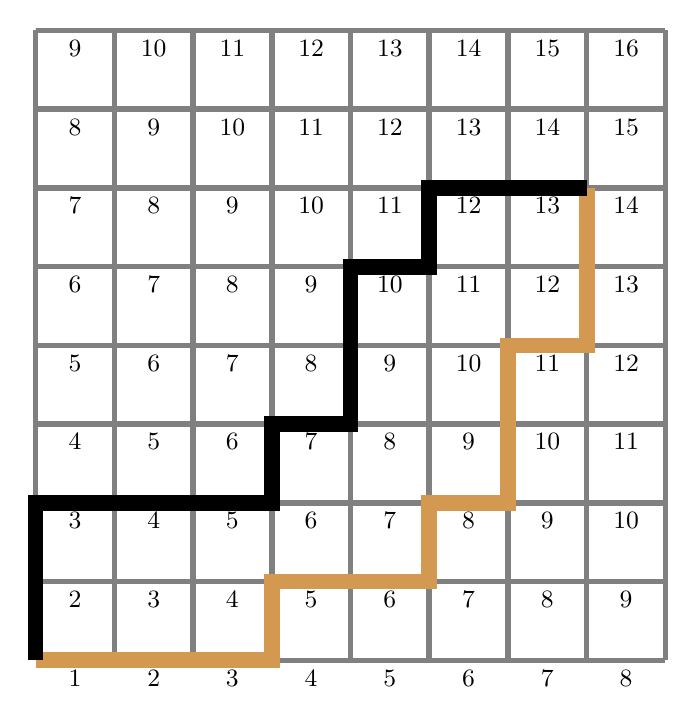
\begin{tikzpicture}
    % Draw the grid
    \foreach \x in {0,1,...,8} {
        \foreach \y in {0,1,...,8} {
            \draw[line width=0.7mm,gray] (\x,0) -- (\x,8); % Vertical lines
            \draw[line width=0.7mm,gray] (0,\y) -- (8,\y); % Horizontal lines
        }
    }
    % Label the East unit segments
    \foreach \x in {0,1,...,7} {
        \foreach \y in {0,1,...,8} {
            \node[below] at (\x+0.5,\y) {\small \the\numexpr\x+\y+1\relax};
        }
    }
     % Blue Path (more southern)
    \draw[line width=2mm, pOrange] 
        (0,0) -- (1,0) -- (2,0) -- (3,0) -- (3,1) -- (4,1) -- (5,1) -- (5,2) -- (6,2) -- (6,3) -- (6,4) -- (7,4) -- (7,5) -- (7,6);
    
    % Red Path (more northern, creating larger gap)
    \draw[line width=2mm, black] 
        (0,0) -- (0,1) -- (0,2) -- (1,2) -- (2,2) -- (3,2) -- (3,3) -- (4,3) -- (4,4) -- (4,5) -- (5,5) -- (5,6) -- (6,6) -- (7,6);

\end{tikzpicture}
\end{document}
